\providecommand{\main}{../../../..}
\documentclass[\main/dresen_thesis.tex]{subfiles}
\begin{document}
  \label{sec:colloidalCrystals:layers:gisaxs}
  \begin{figure}[tb]
    \centering
    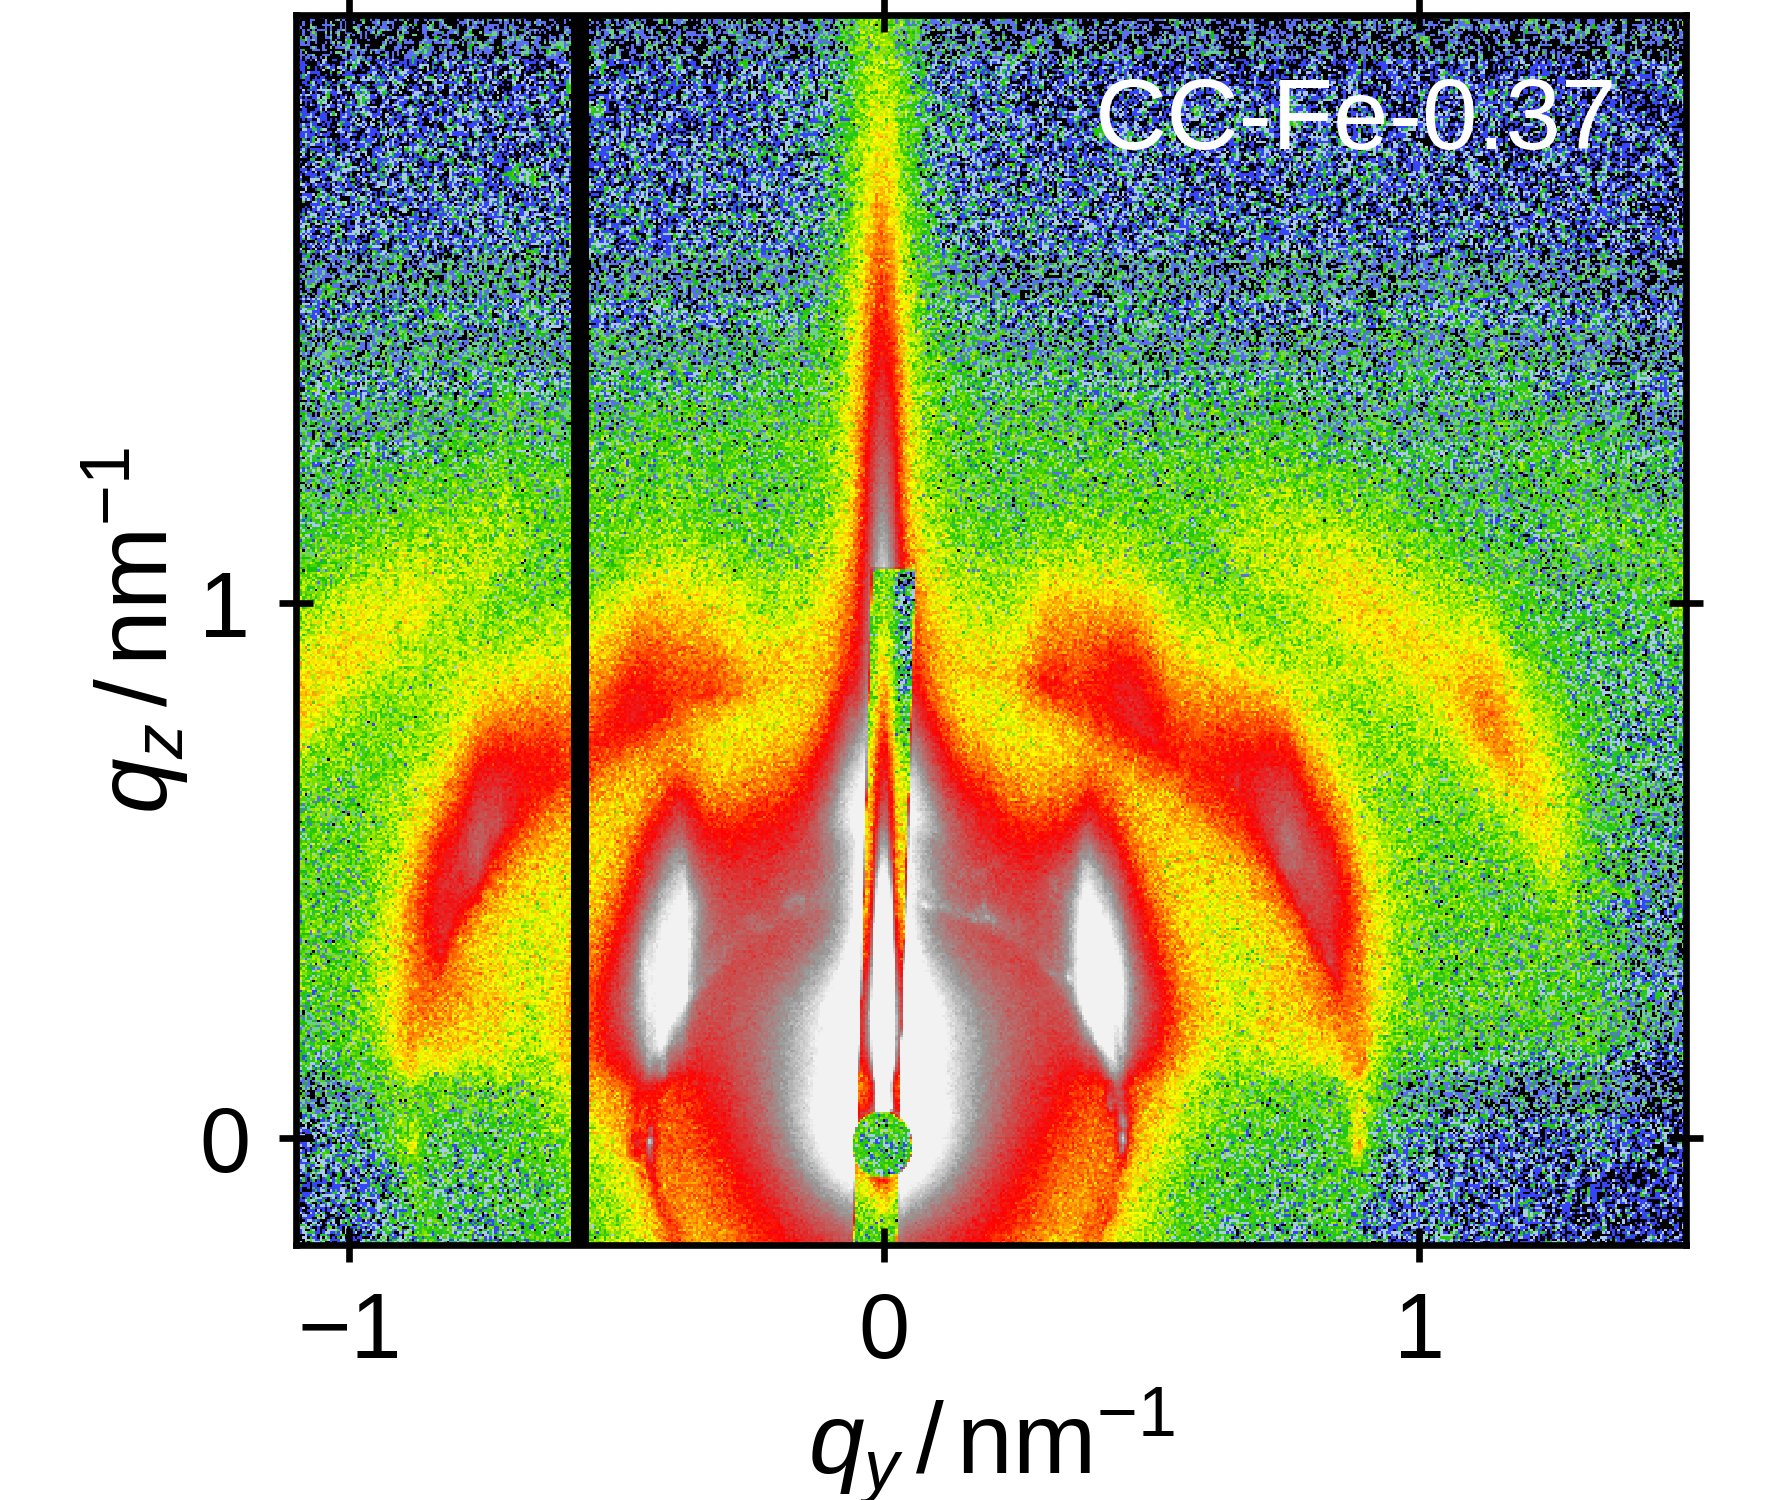
\includegraphics{colloidalCrystals_GISAXS_CC-Fe-0_37}
    \caption{\label{fig:colloidalCrystals:layers:gisaxs}GISAXS of CC-Fe-0.37.}
  \end{figure}
  Write something
  
  % GISAXS is used to estimate the the packing density and average particle-to-particle distance by evaluating the structure factor.
  % In \reffig{fig:looselyPackedNP:layer:gisaxsSC_IOS_11} and \reffig{fig:looselyPackedNP:layer:gisaxsSC_IOS_7} GISAXS experiments for SC-IOS-11 and SC-IOS-7 is shown, as well as the intensity in the Yoneda band and the nanoparticle form factor obtained from SAXS.
  % The GISAXS patterns are in both cases dominated by the form factor of the nanospheres, visible by the rings.
  % Slight modulations of the scattering in the rings are visible, giving rise to a structure factor.
  % Due to the weak intensity of those modulations, the order from the structure factor is short-ranged.
  % \begin{figure}[tb]
  %   \centering
  %   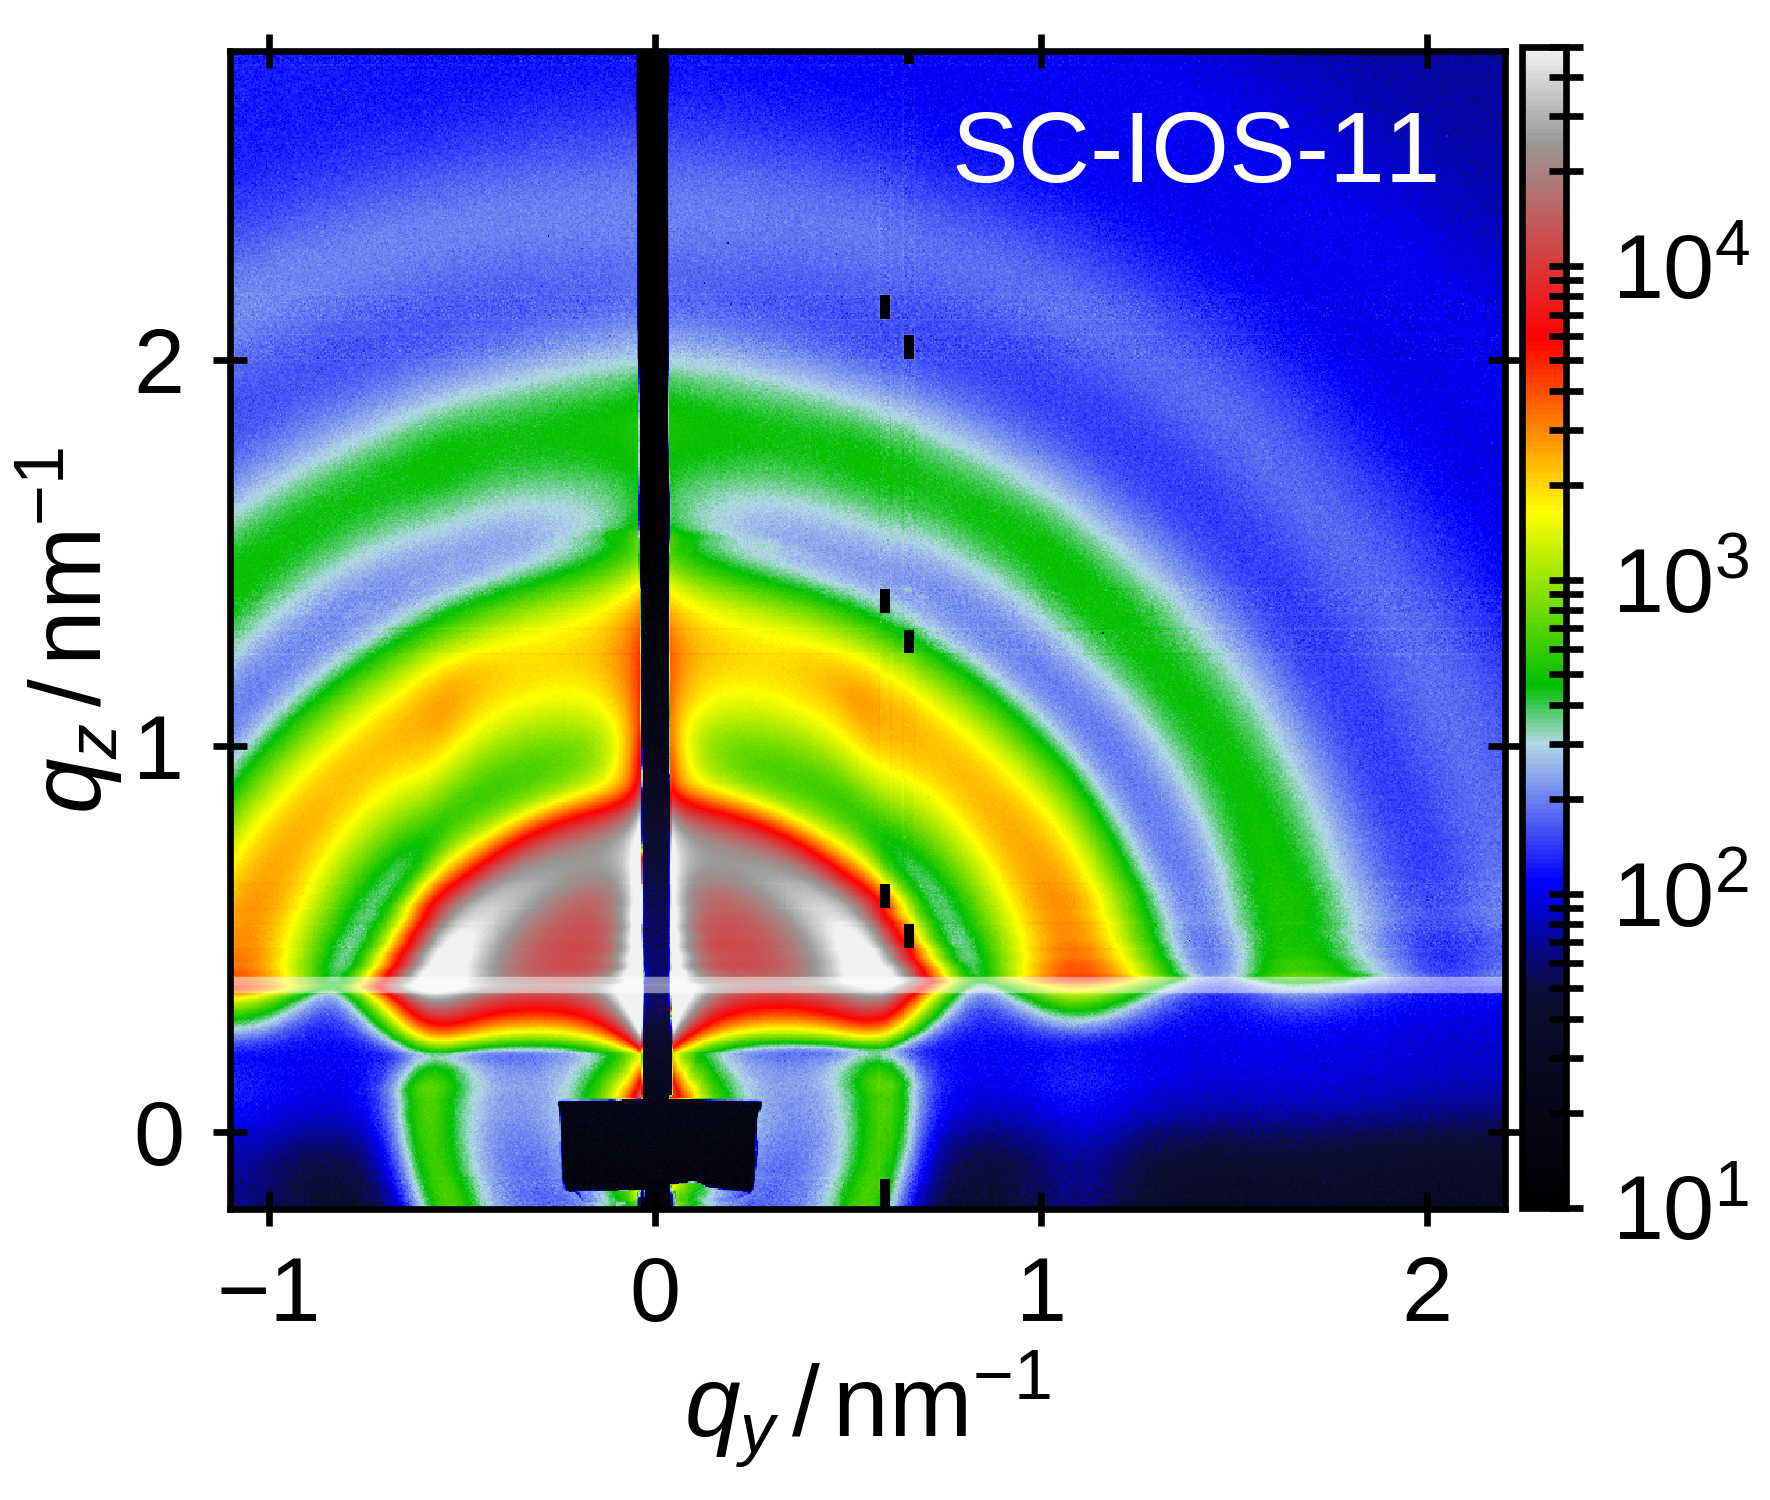
\includegraphics{looselyPackedNP_GISAXS_SC-IOS-11}
  %   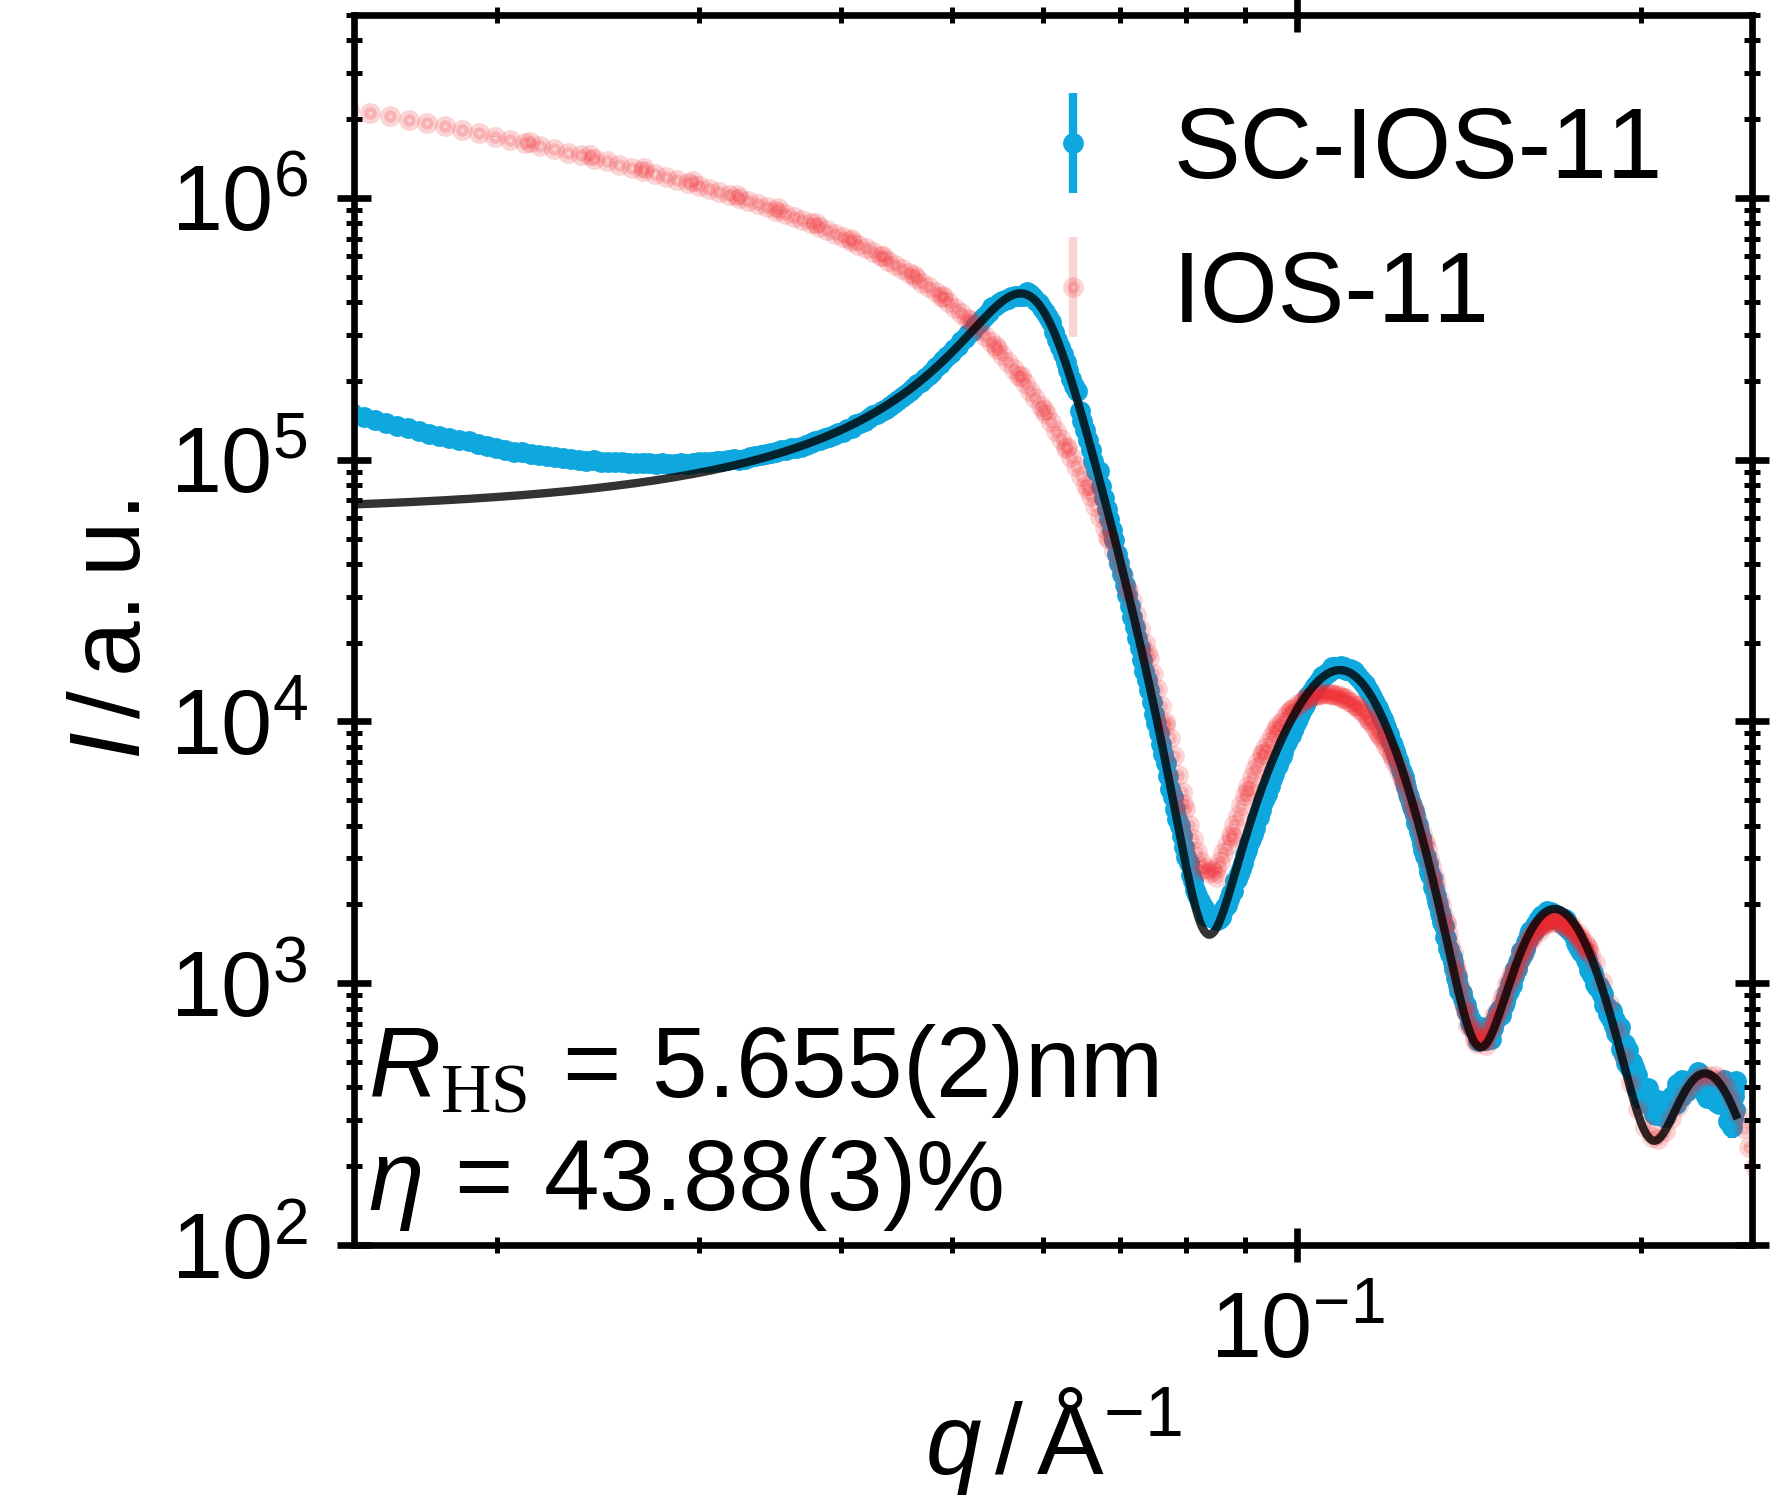
\includegraphics{looselyPackedNP_GISAXS_StructureFactor_SC-IOS-11}
  %   \caption{\label{fig:looselyPackedNP:layer:gisaxsSC_IOS_11}GISAXS detector images (left) of SC-IOS-11 measured under an incident angle of $\alpha_i \eq 0.2 \unit{^\circ}$ and the integrated data in the Yoneda band (right) as blue curve and the previously determined SAXS data (rescaled) for comparison in red. The integrated area for the Yoneda band is shown on the detector image as white stripe. A fit of the intensity using a hard-sphere structure factor in Percus-Yervick approximation, with parameters listed in \reftab{tab:looselyPackedNP:nanoparticle:gisaxs} is shown in black.}
  % \end{figure}

  % By using the parametrization of the form factor from SAXS determined in \refsec{sec:looselyPackedNS:nanoparticle:sas}, a hard-sphere structure factor is determined from the data to quantitatively evaluate the short-range order, which is also shown in \reffig{fig:looselyPackedNP:layer:gisaxs}.
  % At small $q$ values the measured intensity deviates from the product of the structure factor and form factor, due to contributions from the specular reflection, otherwise the measured off-specular scattering on the Yoneda band is well described in both cases.
  % For SC-IOS-11, the hard-sphere radius is determined to $5.655(2) \unit{nm}$ and the packing fraction to $43.88(3) \%$.
  % For SC-IOS-7, a hard-sphere radius of $3.872(4) \unit{nm}$ and packing fraction of $34.20(9) \%$ is observed.
  % \begin{table}[tb]
  %   \centering
  %   \caption{\label{tab:looselyPackedNP:nanoparticle:gisaxs}Parameters for the hard-sphere structure factor in Percus-Yervick approximation shown in \reffig{fig:looselyPackedNP:layer:gisaxs} for both SC-IOS-11 and SC-IOS-7. $R_\mathrm{HS}$ is the hard-sphere radius and $\eta$ the packing fraction of the structure factor. Using both values the Wigner-Seitz radius $\bar{r}$ is determined.}
  %   \begin{tabular}{ c | l | l }
  %     \rule{0pt}{2ex} \textbf{GISAXS}  & \textbf{SC-IOS-11} & \textbf{SC-IOS-7} \\
  %     \hline
  %     \rule{0pt}{2ex} $R_\mathrm{HS} \, / \unit{nm}$          & $5.655(2)$           & $3.872(4)$\\
  %     \rule{0pt}{2ex} $\eta          \, / \unit{\%}$          & $43.88(3)$           & $34.20(9)$\\
  %     \hline
  %     \rule{0pt}{2ex} $\bar{r}       \, / \unit{nm}$          & $7.44(1)$            & $5.54(1)$\\
  %     \hline
  %   \end{tabular}
  % \end{table}
  % % \rule{0pt}{2ex} $I_0           \, / \unit{a.u.}$        & $2550(4)$            & $22405(53)$\\
  % % \rule{0pt}{2ex} $I_\mathrm{bg} \, / \unit{a.u.}$        & $411(10)$            & $147(10)$\\
  % \begin{figure}[tb]
  %   \centering
  %   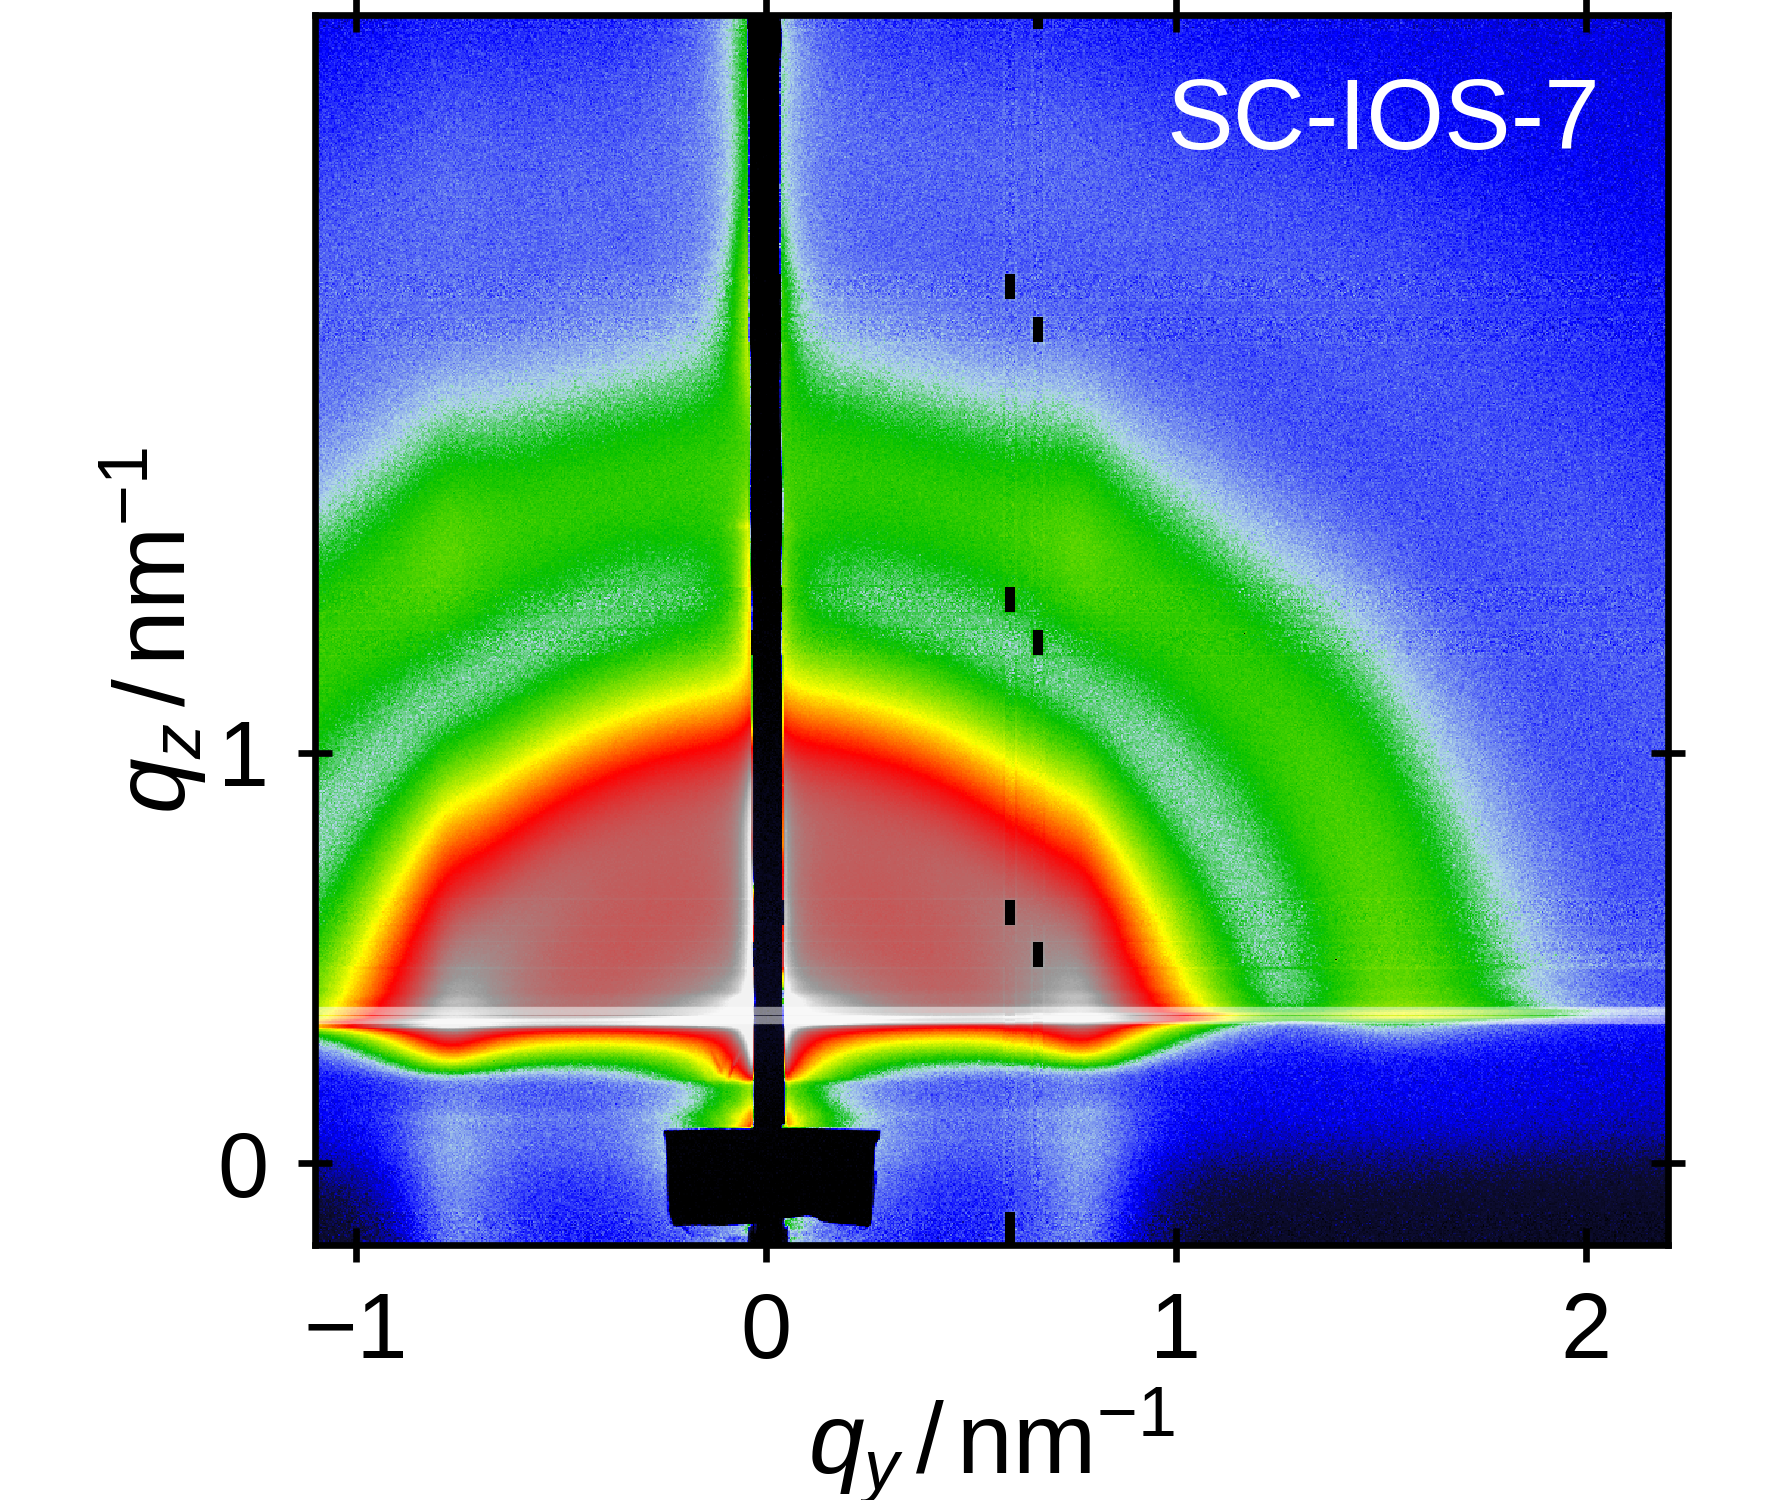
\includegraphics{looselyPackedNP_GISAXS_SC-IOS-7}
  %   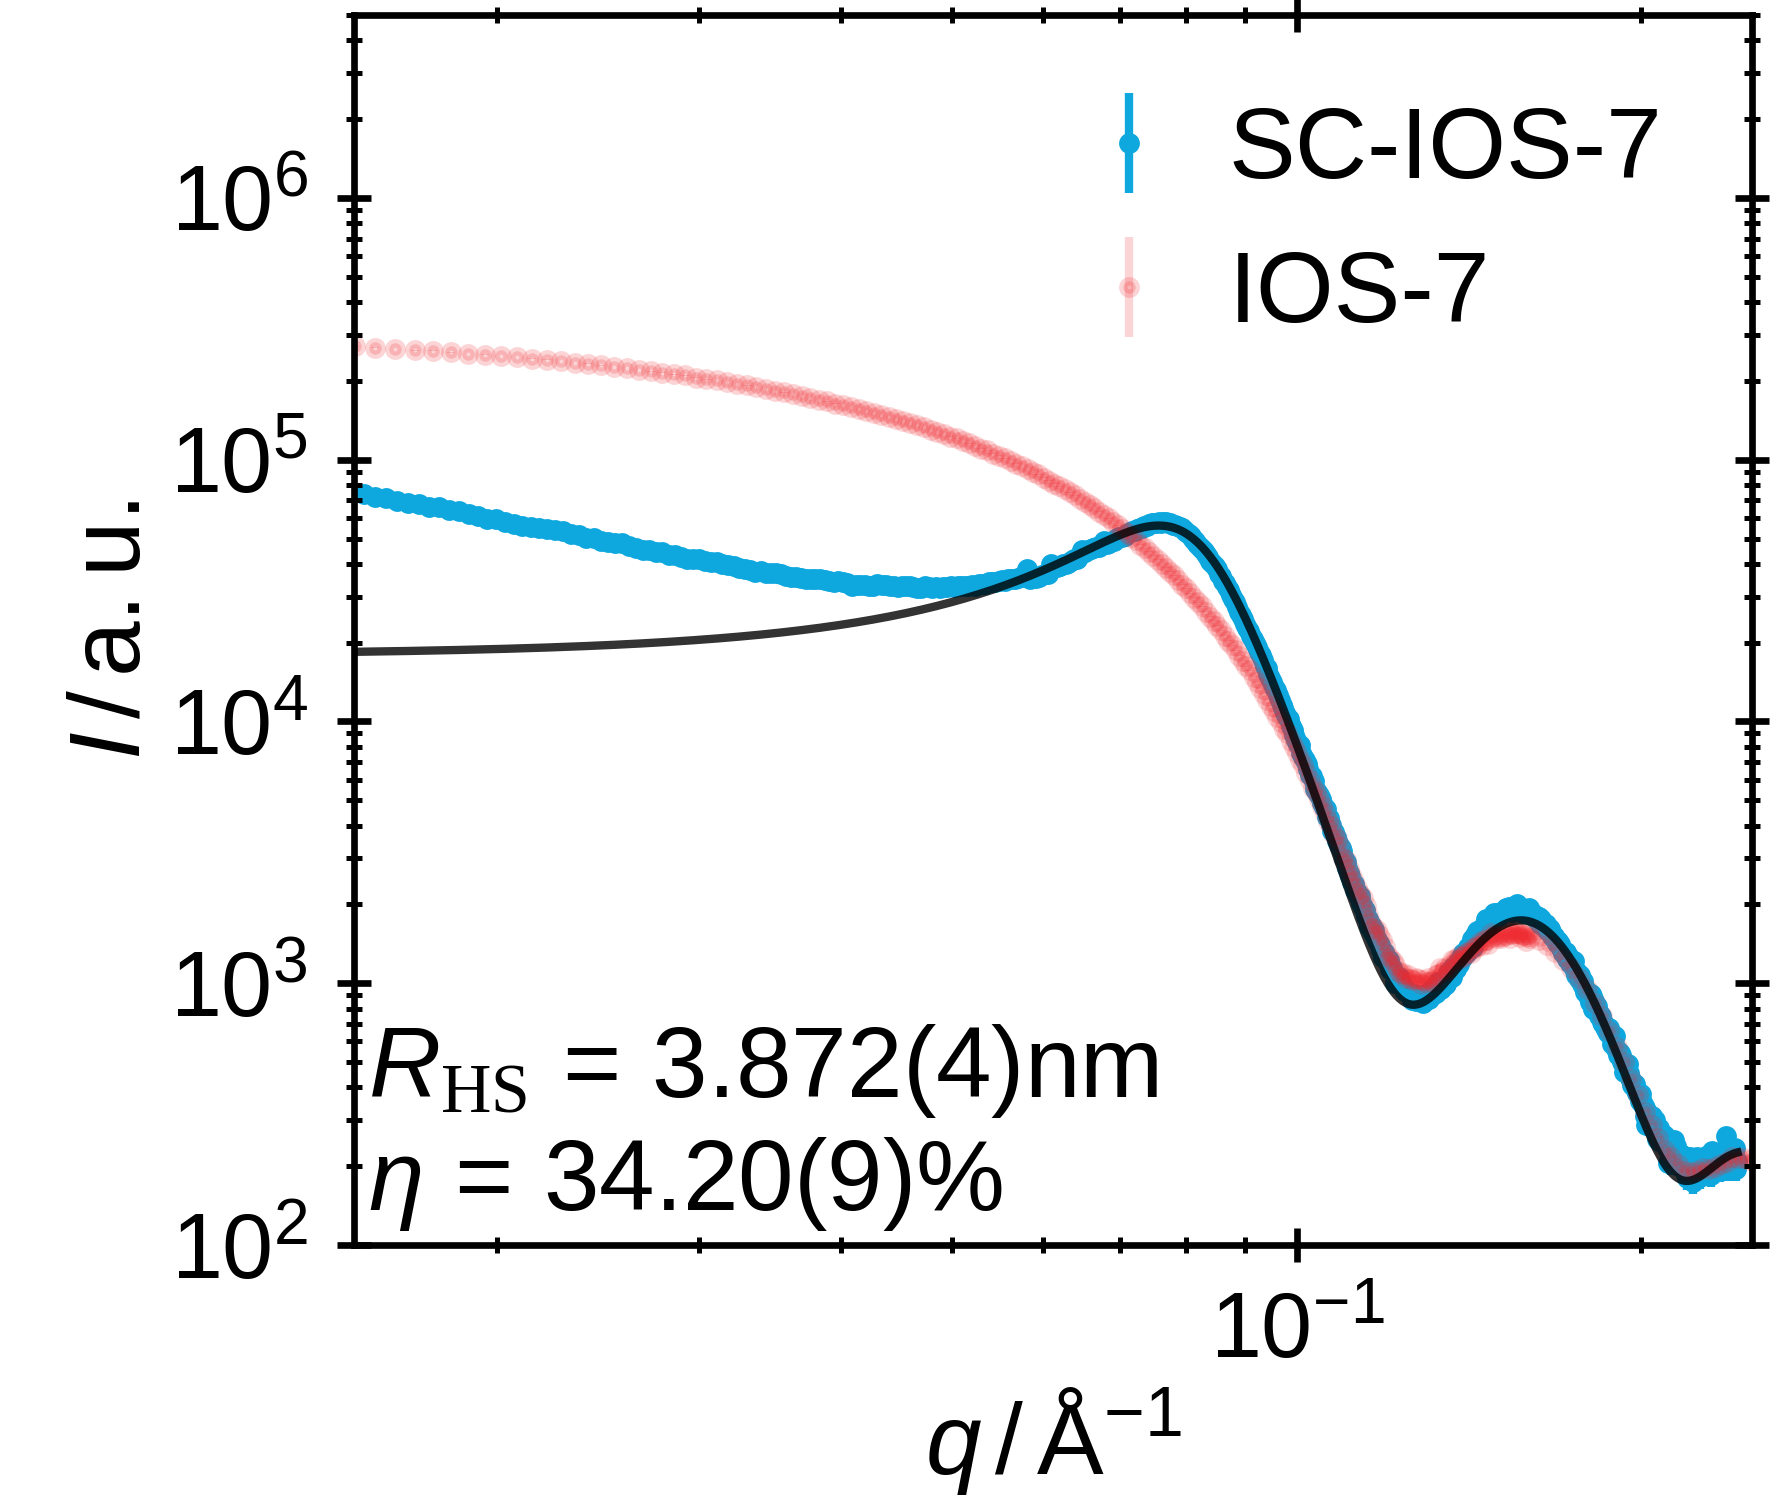
\includegraphics{looselyPackedNP_GISAXS_StructureFactor_SC-IOS-7.png}
  %   \caption{\label{fig:looselyPackedNP:layer:gisaxsSC_IOS_7}GISAXS detector image and evaluation of the structure factor for SC-IOS-7. The measurement and evaluation is analogue to \reffig{fig:looselyPackedNP:layer:gisaxsSC_IOS_11}.}
  % \end{figure}

  % In comparison to the particle radius of IOS-11 and IOS-7 obtained by SAXS ($5.4 \unit{nm}$ and $3.6 \unit{nm}$ respectively), the hard-sphere radius is increased by approximately $0.3 \unit{nm}$ in both cases.
  % This is less than the estimated length of an oleic acid chain, which is in the order of $2.1 \unit{nm}$.
  % This can be interpreted as the particles penetrating the oleic acid shells of one another, and that the oleic acid shells do not act as hard repulsive shells as is the assumption for the hard-sphere radius in the used structure factor.

  % The packing fractions on the other hand are strongly reduced in comparison to a dense spherical packing ($\pi / \sqrt(18) \approx 74 \%$).
  % The observed values are even lower than the expected packing density for loosely random packed spheres ($58 \%$ \cite{Tory_1973_Simul, Shi_2008_Simul}).
  % This suggests that additional voids are present in the particle layer and that particles have on average a larger spacing than the hard-sphere radius.
  % Estimating the average particle spacing by the Wigner-Seitz radius $\bar{r}$, which given by the inverse of the particle number density
  % \begin{align}
  %   \begin{split}
  %     \frac{4 \pi}{3} \bar{r}^3 &\eq \frac{V}{N}\\
  %     \Rightarrow \bar{r}       &\eq \frac{R_\mathrm{HS}}{\sqrt[3]{\eta}},
  %   \end{split}
  % \end{align}
  % a mean Wigner-Seitz radius of $7.44 \unit{nm}$ is obtained for SC-IOS-11 and $5.54 \unit{nm}$ for SC-IOS-7.
  % These values are approximately $2 \unit{nm}$ larger than the particle radius obtained by SAXS.
  % This can be interpret as that on average the particles are separated by their oleic acid shells and each particle is given exactly the space for its core and surfactant shell.

  % In conclusion, the GISAXS evaluation is giving information on both, the minimum distance the nanoparticles approach eith other via the hard-sphere radius, and the average particle density 

\end{document}